%%%%%%%%%%%%%%%
% This bachelor's/master's degree thesis style is based of already applied MS Word template in the
% Faculty of Electrical Engineering and Electronics of Technical University Gabrovo.
% Author: Svetlozar Kosev
% Last modified: 24 June 2023
%%%%%%%%%%%%%%%
\documentclass[11pt, a4paper]{article}
%\documentclass[11pt,a4paper,twoside]{article}

\usepackage[T2A]{fontenc}
\usepackage[utf8]{inputenc}
\usepackage[bulgarian, english]{babel}
%\setmainfont{Times New Roman}

\renewcommand{\listoffigures}{Списък на фигури}


\setcounter{tocdepth}{4} %sections + subsections in the TOC
\addto{\captionsenglish}{ 
	\renewcommand*{\contentsname}{Съдържание} 
	\renewcommand*{\figurename}{Фигура} 
	\renewcommand*{\tablename}{Таблица} 
	\renewcommand*{\refname}{Библиография} 
	\renewcommand*{\appendixname}{Приложение} 
	}
	
%\renewcommand{\listfigurename}{Списък на фигури}

%Put here the other needed macro packages.
\usepackage{graphicx} %for the raster graphics
\usepackage[warn]{
	textcomp
} %for the degree (\textdegree) and number (\textnumero) sign
\usepackage{hyperref} %for the URLs
\usepackage{hyphenat} %for hyphenation of words containing hyphen
\usepackage{fancyhdr} %for the headers design
\usepackage[
headheight=22pt,
top=1.50cm,
bottom=1.80cm,
left=2.50cm,
right=2.50cm,
includeheadfoot
]{geometry} % Use similar margins to the Word Template


%\fancypagestyle{body}{
	%	\fancyhf{}
	%	\fancyhead[LE,RO]{Раздел \textbf{\nouppercase{\leftmark}}}
	%	\fancyhead[RE,LO]{\thepage}
	%}
%\fancypagestyle{contents}{
	%	\fancyhf{}
	%	\fancyhead[LE,RO]{\thepage}
	%	\fancyhead[RE,LO]{\leftmark}
	%	\renewcommand{\headrulewidth}{1.0pt}
	%	\renewcommand{\footrulewidth}{1.0pt}
	%}
%\fancypagestyle{introduction}{
	%	\fancyhf{}
	%	\fancyhead[LE,RO]{\thepage}
	%	\fancyhead[RE,LO]{\leftmark}
	%	\renewcommand{\headrulewidth}{1.0pt}
	%	\renewcommand{\footrulewidth}{1.0pt}
	%}
%\fancypagestyle{appendix}{
	%	\fancyhf{}
	%	\fancyhead[LE,RO]{\thepage}
	%	\fancyhead[RE,LO]{Приложения}
	%	\renewcommand{\headrulewidth}{1.0pt}
	%	\renewcommand{\footrulewidth}{1.0pt}
	%}

% Begin the actual document
\begin{document}
	%	\pagestyle{body}	
	% Define the page styles
\fancypagestyle{titlepage}{
	\pagestyle{empty}
	\fancyhf{}
	\fancyhead[C]{\LARGE{\textbf{Технически университет – Габрово}}}
	\renewcommand{\headrulewidth}{1.5pt}
	\renewcommand{\footrulewidth}{1.5pt}
	\fancyfoot[C]{} % Remove the center footer content (page number)
}

%\clearpage
\pagestyle{titlepage}
%\pagestyle{empty}

\title{}
\date{\vspace{-18ex}}
\maketitle

\begin{center}
	{
\includegraphics[width=3cm]{images/logo.jpg}\\ \huge{\textbf{Факултет „Електроника и електротехника”}}\\ \huge{\textbf{Катедра „Компютърни системи и технологии”}}\\ \vspace*{0.5cm} \Large{\textbf{Специалност: „Компютърни системи и технологии”,}}\\
		%\Large{\textbf{Магистърска програма по "Метеорология"}}\\
		\vspace*{1.5cm} \Huge{\textbf{Дипломна работа}}\\ \Large{\textbf{за}}\\ \Large{\textbf{придобиване на образователно-квалификационна степен „магистър”}}\\ \Large{\textbf{на}}\\ \Large{\textbf{инж. Светлозар В. Косев, факултетен \textnumero\ 21605006}}\\ \vspace*{0.7cm}
		%    \Huge{\textbf{Тема: „Изграждане и мигриране към локална сървърна инфраструктура с HPE ProLiant ML350 Gen10 и Windows Server 2016 Standard “}}\\
		\huge{\textbf{Тема: „Изграждане и мигриране към локална сървърна инфраструктура с HPE ProLiant ML350 Gen10 и Windows Server 2016 Standard”}}\\ \vspace*{1cm} \begin{flushleft}\large{\textbf{Ръководител катедра:}}\hspace{3cm} \large{\textbf{Научен ръководител:}}\end{flushleft} \begin{flushright}
			% Change the \hspace argument depending of the names length.
			\Large{\textbf{\slash доц. Валентина Кукенска \slash}}\hspace{4cm} \Large{\textbf{\slash доц. Делян Генков \slash}}\end{flushright}
		%\begin{flushleft}
		
		% \Large{\textbf{Консултант:}}\\
		
		%\hspace{5cm}\Large{\textbf{/Eжко Бежко/}}
		
		%\end{flushleft}
		\vspace*{1.7cm} \Large{Габрово, 2021} }
\end{center}	
	\newpage
	\clearpage	
	\tableofcontents
	\newpage
	\listoffigures
		\newpage
		\listoftables
			\newpage
	
	% Hence we utilize the article document class and 'Section' higher level partitioning,
	% rather than 'report'/'Chapter', \input is more suitable than \include.
	%	\clearpage
	%	\thispagestyle{empty}
	%%%%%%%%%%%%%%%
% This bachelor's/master's degree thesis style is based of already applied MS Word template in the 
% Faculty of Electrical Engineering and Electronics of Technical University Gabrovo.
% Author: Svetlozar Kosev
% Last modified: 24 June 2023
%%%%%%%%%%%%%%%

\clearpage
\thispagestyle{empty}


%\thispagestyle{introduction}
%\clearpage
%\thispagestyle{empty}
%\markboth{Въведение}{Introduction}
\addcontentsline{toc}{section}{Въведение}

Сървърът е софтуер/операционна система на устройство, което осигурява услуга на друга програма или потребител. В център за данни (data center), физическата машина, на която се изпълнява програма, често се нарича сървър.
		
		\begin{figure}[h]
			\centering
			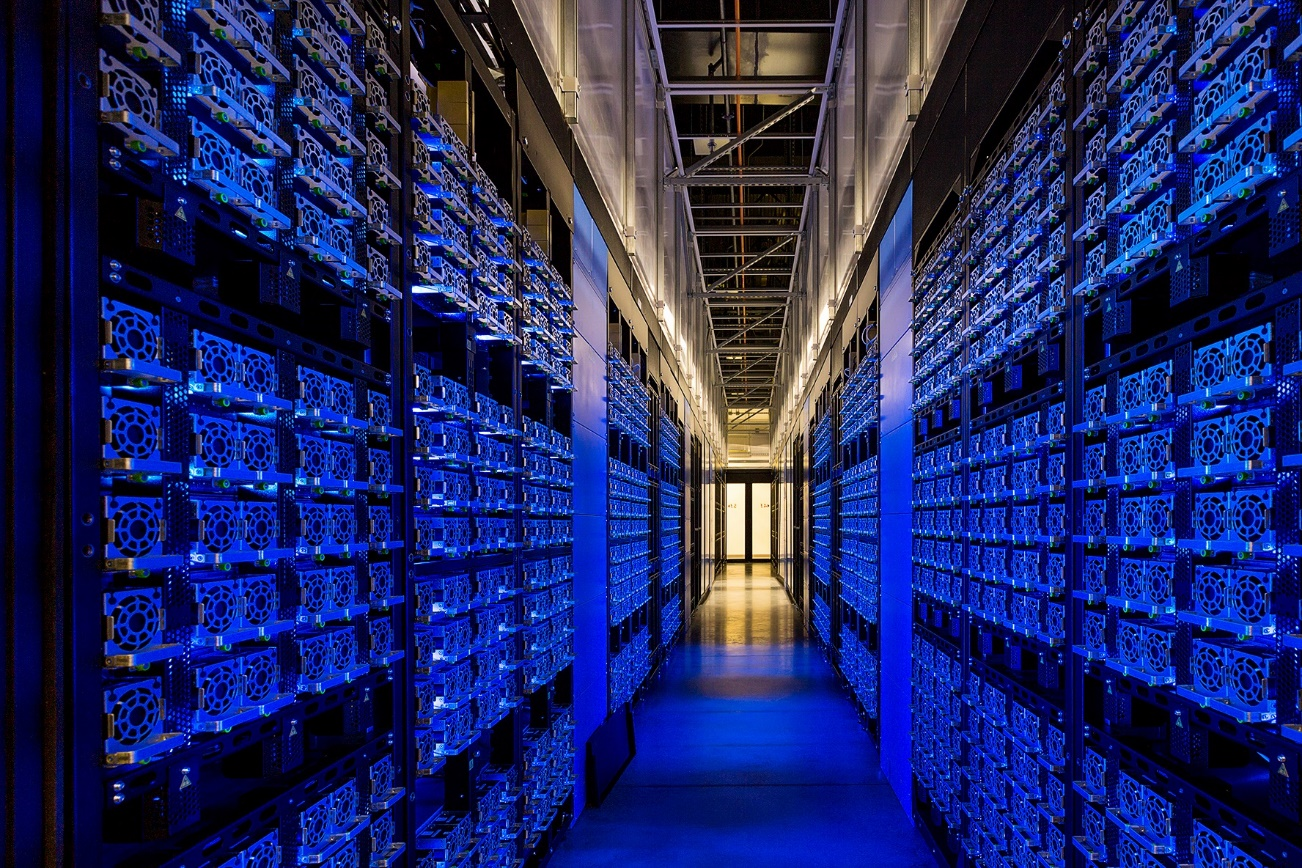
\includegraphics[width=0.8\linewidth]{images/1-1-1Център за данни.png} % replace "example-image" with the filename of your image
			\caption{Център за данни}
			\label{fig:Център за данни}
		\end{figure}
		
		
В моделът клиент-сървър, сървърната програма изчаква и изпълнява заявки от клиентски програми, които могат да се изпълняват в същото време и на други компютри. Някои приложения могат да служат като клиентската програма, с изисквания за услуги, а други – като сървър на заявки от други програми.

Сървърите могат да бъдат както обикновени компютри, така и реално физически или виртуални сървъри със специфичен хардуер и софтуер. Физическия сървър е машина, която се използва за изпълнението на необходим софтуер от клиентите. В повечето случаи, виртуалният сървър е операционна система, инсталирана и конфигурирана с помощта на софтуер за виртуализация. Този тип виртуализация се нарича софтуерна виртуализация (type 2 hypervisor). Популярни софтуери за виртуализация са VirtualBox, VMware Player, KVM, vSphere, QEMU. Изискванията за конфигуриране на виртуализация са процесорът (Intel и AMD) и UEFI/BIOS-ът да я поддържат. (\textit{\textbf{mldunbound.org, 2019}})

		\begin{figure}[h]
	\centering
	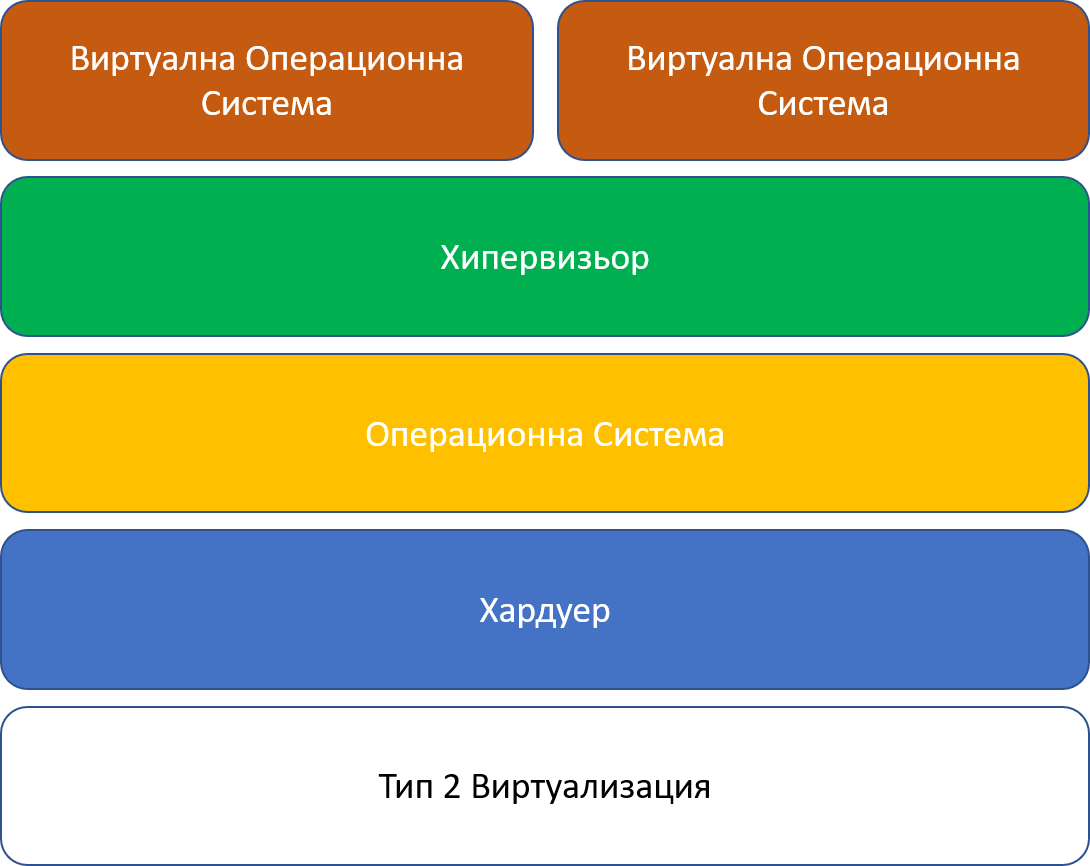
\includegraphics[width=0.8\linewidth]{images/hypervisor2.png} % replace "example-image" with the filename of your image
	\caption{Тип 2 виртуализация}
	\label{fig:Тип 2 виртуализация}
\end{figure}

Другият вид виртуализация е хардуерна (type 1 hypervisor). След като се стартира физическия сървър с инсталиран виртуализатор, се показва екран, приличащ на терминал. Показват се данни за процесора, паметта, мястото за съхранение, IP и MAC адресите. Тук, най-често се използват Hyper-V, Citrix XenServer и VMware ESX.



	{Въведение}\label{Introduction}
	%\input{abstract}
	\newpage
	
	\chapter{Виртуални машини}\label{Sect1}
Текст за Глава 1.
\section{1}
\section{2}
\subsubsection{2.1}
	{Виртуални машини}\label{Sect1}
	%\input{Section1}
	\newpage
	
	\chapter{Предишна инфраструктура, изследване и подготовка}\label{Sect2}

Текст за Глава 2.

\section{aaa}
\section{bbbb}
\subsubsection{cccc}
	{Предишна инфраструктура, изследване и подготовка}\label{Sect2}
	%\input{Section2}
	\newpage
	
	\chapter{Изисквания за нова инфраструктура}\label{Sect3}
Текст за Глава 3.
	{Изисквания за нова инфраструктура}\label{Sect3}
	%\input{Section3}
	\newpage
	
	\chapter{Проектиране на нова инфраструктура}\label{Sect4}
Текст за Глава 4.
	{Проектиране на нова инфраструктура}\label{Sect4}
	%\input{Section4}
	\newpage
	
	\chapter*{Речник на термини}\label{Sect5}

Текст
	{Речник на термини}\label{Sect5}
	%\input{Section5}
	\newpage
	
	\include{abstract/Bibliography.tex}
	{Използвана Литература}\label{Sect7}
	%\input{Section7}
	\newpage
	
	\include{abstract/Acknowledgments.tex}
	\label{Ackn}
	
	\newpage
	%\section*{Благодарности}\{Ackn}
%\input{Acknowledgements}
%\newpage
%\pagestyle{contents}

%\section*{Благодарности}\{Ackn}
%\input{Acknowledgements}
%\newpage

%\pagestyle{contents}

%\input{thebiblography}
\end{document}